%!TEX program = xelatex
\documentclass[9pt, compress]{beamer}
\usetheme[titleprogressbar]{m}

\usepackage{array}
\usepackage{tabu}
\usepackage[english,russian]{babel} 
\usepackage{longtable} %tabu needs this to be loaded.
\usepackage{lipsum}

\usepackage{rotating}
\usepackage{graphicx}
\usepackage{color}
\usepackage{xcolor}
\usepackage{listings}
\usepackage{sectsty}
\usepackage{caption}


\DeclareCaptionFont{white}{\color{white}}
\DeclareCaptionFormat{listing}{\colorbox{gray}{\parbox{\dimexpr\textwidth-1.72\fboxsep\relax}{#1#2#3}}}
\captionsetup[lstlisting]{format=listing,labelfont=white,textfont=white,margin=0pt}
\lstset{language=C,
	basicstyle=\footnotesize,
	keepspaces=true,
	numbers=left,
	tabsize=4,               
	frame=single,                           % Single frame around code
	rulecolor=\color{black},
	captionpos=b,
	showstringspaces=false,	
	abovecaptionskip=-0.9pt,
	xleftmargin=3.4pt,
	xrightmargin=2.6pt,
	breaklines=true,
	postbreak=\raisebox{0ex}[0ex][0ex]{\ensuremath{\color{black}\hookrightarrow\space}},
	xleftmargin=3.2pt,
	literate={а}{{\selectfont\char224}}1
	{~}{{\textasciitilde}}1
	{б}{{\selectfont\char225}}1
	{в}{{\selectfont\char226}}1
	{г}{{\selectfont\char227}}1
	{д}{{\selectfont\char228}}1
	{е}{{\selectfont\char229}}1
	{ё}{{\"e}}1
	{ж}{{\selectfont\char230}}1
	{з}{{\selectfont\char231}}1
	{и}{{\selectfont\char232}}1
	{й}{{\selectfont\char233}}1
	{к}{{\selectfont\char234}}1
	{л}{{\selectfont\char235}}1
	{м}{{\selectfont\char236}}1
	{н}{{\selectfont\char237}}1
	{о}{{\selectfont\char238}}1
	{п}{{\selectfont\char239}}1
	{р}{{\selectfont\char240}}1
	{с}{{\selectfont\char241}}1
	{т}{{\selectfont\char242}}1
	{у}{{\selectfont\char243}}1
	{ф}{{\selectfont\char244}}1
	{х}{{\selectfont\char245}}1
	{ц}{{\selectfont\char246}}1
	{ч}{{\selectfont\char247}}1
	{ш}{{\selectfont\char248}}1
	{щ}{{\selectfont\char249}}1
	{ъ}{{\selectfont\char250}}1
	{ы}{{\selectfont\char251}}1
	{ь}{{\selectfont\char252}}1
	{э}{{\selectfont\char253}}1
	{ю}{{\selectfont\char254}}1
	{я}{{\selectfont\char255}}1
	{А}{{\selectfont\char192}}1
	{Б}{{\selectfont\char193}}1
	{В}{{\selectfont\char194}}1
	{Г}{{\selectfont\char195}}1
	{Д}{{\selectfont\char196}}1
	{Е}{{\selectfont\char197}}1
	{Ё}{{\"E}}1
	{Ж}{{\selectfont\char198}}1
	{З}{{\selectfont\char199}}1
	{И}{{\selectfont\char200}}1
	{Й}{{\selectfont\char201}}1
	{К}{{\selectfont\char202}}1
	{Л}{{\selectfont\char203}}1
	{М}{{\selectfont\char204}}1
	{Н}{{\selectfont\char205}}1
	{О}{{\selectfont\char206}}1
	{П}{{\selectfont\char207}}1
	{Р}{{\selectfont\char208}}1
	{С}{{\selectfont\char209}}1
	{Т}{{\selectfont\char210}}1
	{У}{{\selectfont\char211}}1
	{Ф}{{\selectfont\char212}}1
	{Х}{{\selectfont\char213}}1
	{Ц}{{\selectfont\char214}}1
	{Ч}{{\selectfont\char215}}1
	{Ш}{{\selectfont\char216}}1
	{Щ}{{\selectfont\char217}}1
	{Ъ}{{\selectfont\char218}}1
	{Ы}{{\selectfont\char219}}1
	{Ь}{{\selectfont\char220}}1
	{Э}{{\selectfont\char221}}1
	{Ю}{{\selectfont\char222}}1
	{Я}{{\selectfont\char223}}1,
	extendedchars=true
}
\usepackage{textpos}
\newcommand<>{\fullsizegraphic}[1]{
  \begin{textblock*}{0cm}(-1cm,-3.78cm)
  \includegraphics[width=\paperwidth]{#1}
  \end{textblock*}
}

%галочка
\usepackage{amssymb}% http://ctan.org/pkg/amssymb
\usepackage{pifont}% http://ctan.org/pkg/pifont
\newcommand{\cmark}{\ding{52}}%
\newcommand{\xmark}{\ding{56}}


\usepackage{booktabs}  
\usepackage[scale=2]{ccicons}
\usepackage{minted}
\usepgfplotslibrary{dateplot}
\usemintedstyle{trac}
\author{Студент: \textbf{Д.В. Круминьш}\\ 
	Группа: \textbf{13541/3}\\ \\
	Преподаватель: \textbf{Е.В. Душутина} }
\title{Системные вызовы}
\subtitle{Курс: \textbf{Проектирование ОС и компонентов}}
%\logo{123}
\institute{Санкт-Петербургский политехнический университет Петра Великого}
\date{ }
%\subject{}
%\setbeamercovered{transparent}
%\setbeamertemplate{navigation symbols}{}
\begin{document}
	\maketitle
%	\begin{frame}
%		\frametitle{Оглавление}
%		\tableofcontents{}
	%\end{frame}
	

\begin{frame}
\frametitle{Рассматриваемые системные вызовы}
Рассматриваемые системные вызовы: \textbf{fork, execve, exit}.

В работе рассматриваются следующие версий ядер:
\begin{itemize}
\item \textbf{4.13.0-38-generic} - \textbf{Ubuntu 16.04};
\begin{itemize}
\item glibc 2.23
\end{itemize}
\item \textbf{2.6.32-21-generic} - \textbf{Ubuntu 10.04}
\begin{itemize}
\item glibc 2.11.1
\end{itemize}
\end{itemize}
Для выполнения работы использовалась \textbf{VMware Workstation 12 pro (12.5.7 build-5813279)}
\end{frame}


\section{Перехват системных вызовов}
\begin{frame}
\frametitle{Принцип перехвата}
Перехват будет осуществляться для версии ядра 2.6.32-21, с использованием:
\begin{itemize}
\item \textbf{LKM} (Linux loadable kernel module) - динамическое подключения/отключения модулей ядра без перекомпиляции всего ядра.
\item \textbf{Отображение в память} системной функции с модифицированным прологом, ссылающимся на функцию перехватчик.
\end{itemize}
\end{frame}

\begin{frame}
\frametitle{Схема перехвата}
\begin{center}
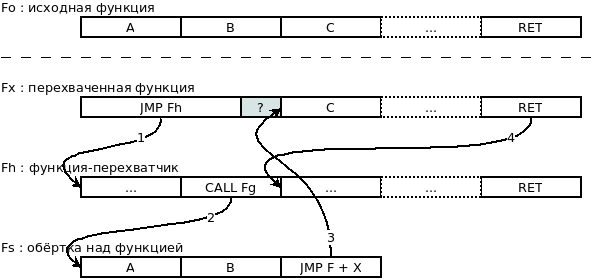
\includegraphics[width=\textwidth]{img/hookScheme}
\end{center}
\end{frame}



\begin{frame}
\frametitle{Сложности перехвата на новых версиях ядер}
С ядра версии 2.6, активно началась защита ядра от внешних воздействий, многие функции были убраны из экспорта.

Возможный перехват:
\begin{enumerate}
\item \textbf{LSM} - фреймворк для разработки модулей безопасности ядра. Перед обращением ядра к внутреннему объекту будет обязательно вызвана функция проверки, предоставленная LSM. К сожалению предоставляет возможность перехвата не для всех системных вызовов.
\item \textbf{Полная перекомпиляция ядра} с внесением изменений, для обеспечения возможности перехвата.
\end{enumerate}
\end{frame}


\section{Системная функция fork}
\begin{frame}
\frametitle{Описание}
\textbf{fork()} - системный вызов, создающий новый процесс (потомок), который является практически полной копией процесса-родителя, выполняющего этот вызов. Дочерний и родительский процессы находятся в отдельных пространствах памяти.  Создавшийся процесс будет занят выполнением того же кода ровно с той же точки, что и исходный процесс.\\
\textbf{Расположение: }.../kernel/fork.c\\
\textbf{Синтаксис: }long sys\_fork(struct pt\_regs *regs)\\\\
В виде параметра выступает указатель на структуру с регистрами, возращаемое значение - id процесса потомка.
\end{frame}

\begin{frame}[fragile]
\frametitle{Программы для анализа}
\lstinputlisting[firstnumber=8,firstline=8,lastline=12,caption=Использование функции fork из glibc, language=C, label={lst:fork1}]{sourceCode/fork/programs/forkExample.c}
\lstinputlisting[caption=Прямой вызов системной функции, language=C, label={lst:fork2}]{sourceCode/fork/programs/fork2.c}
\end{frame}	


\begin{frame}[fragile]
\frametitle{[Ядро 4.13.0][FORK] STRACE}
\lstinputlisting[firstnumber=18,firstline=18,lastline=27, caption=Использование функции fork из glibc]{sourceCode/fork/kernel_4.13/forkStrace.log}
По части лога видно, что сперва происходит отображение в память, а затем и создание нового процесса. Однако создание нового процесса было произведено с помощью системной функции clone(), а не fork().
\end{frame}	


\begin{frame}[fragile]
\frametitle{[Ядро 4.13.0][FORK] STRACE}
\lstinputlisting[firstnumber=26,firstline=26,lastline=32, caption=Прямой вызов системной функции, label={lst:trueFork}]{sourceCode/fork/kernel_4.13/fork2Strace.log}
Strace показал, что теперь, действительно был вызван систмный вызов \textbf{fork}, который вернул значение 7724.
\end{frame}	


\begin{frame}[fragile]
\frametitle{[Ядро 4.13.0] Таблица системных вызовов}
Таблица представлена в виде:
\begin{center}
\textbf{<number> <abi> <name> <entry point>}
\end{center}
\textbf{number} - уникальный номер системного вызова\\
\textbf{abi} - интерфейс для использования\\
\textbf{name} - название системного вызова\\
\textbf{entry point} - входная точка
\lstinputlisting[firstnumber=63,firstline=63,lastline=69, caption=.../arch/x86/syscalls/syscall\_64.tbl, label={lst:64tbl}]{sourceCode/kernel/4.13/arch/x86/entry/syscalls/syscall_64.tbl}
\end{frame}	

\section{Анализ glibc}
\begin{frame}[fragile]
\frametitle{[Ядро 4.13.0] Анализ glibc}
Проанализируем исходный код glibc, в данном случае программы компилировались используя \textbf{glibc 2.23}.\\\\
По пути \textbf{glibc\_2.23/sysdeps/nptl/fork.c} имеется файл fork.c, в котором в строках 124-129 и представлен вызов функции.
\lstinputlisting[firstnumber=124,firstline=124,lastline=129, caption=glibc\_2.23/sysdeps/nptl/fork.c]{sourceCode/fork/glibc/2.23/sysdeps/nptl/fork.c}

\end{frame}	

\begin{frame}[fragile]
\frametitle{[Ядро 4.13.0] Анализ glibc}
Реализация макроса представлена по пути \textbf{glibc\_2.23/sysdeps/unix/sysv/linux/x86\_64/arch-fork.h} в файле arch-fork.h.
\lstinputlisting[firstnumber=24,firstline=24,lastline=27, caption=glibc\_2.23/sysdeps/unix/sysv/linux/x86\_64/arch-fork.h]{sourceCode/fork/glibc/2.23/sysdeps/unix/sysv/linux/x86_64/arch-fork.h}

Как видно из реализации макроса, вызывается системный вызов clone(), а не fork().
\end{frame}	

\begin{frame}[fragile]
\frametitle{[Ядро 4.13.0][FORK] Анализ исходного кода}
Исходный код(основная часть), находится в файле \textbf{fork.c}, по пути \textbf{/kernel}.
\lstinputlisting[firstnumber=2006,firstline=2006,lastline=2012, caption=.../kernel/fork.c]{sourceCode/kernel/4.13/kernel/fork.c}
\begin{itemize}
\item \textbf{clone\_flags} - флаг, для определения того, что именно нужно копировать;
\item \textbf{parent\_tid и child\_tid} - два указателя в пространстве пользователя, для хренения id родительского и дочернего процессов;
\item \textbf{stack\_start} - адрес начала стека с процессами;
\item \textbf{tls} - определение локального хранилища для нового процесса
\end{itemize}
\end{frame}	


\begin{frame}[fragile]
\frametitle{[Ядро 4.13.0][FORK] Схема работы do\_fork}
\begin{figure}[H]
  \centering
  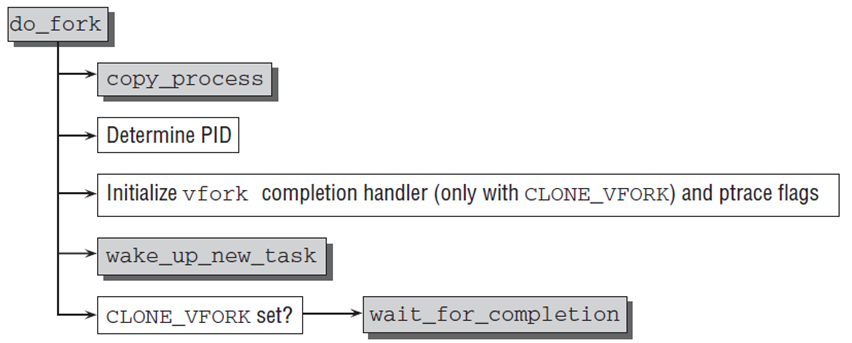
\includegraphics[width=\textwidth]{img/do_fork}
  \caption*{Схема работы do\_fork}
  \captionsetup{labelformat=empty}
\end{figure}
\end{frame}	


\begin{frame}[fragile]
\frametitle{[Ядро 4.13.0][FORK] Схема работы copy\_process}
\begin{figure}[H]
  \centering
  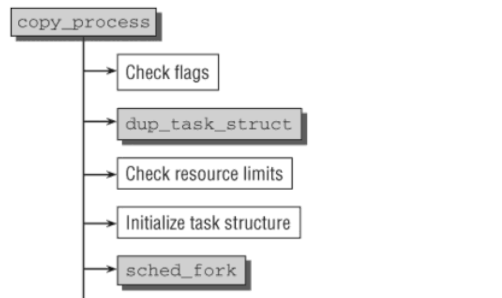
\includegraphics[width=.9\textwidth]{img/copy_process}
  \caption*{Схема работы copy\_process}
\end{figure}
\end{frame}	

\begin{frame}[fragile]
\frametitle{[Ядро 4.13.0][FORK] Схема работы copy\_process}
\begin{figure}[H]
  \centering
  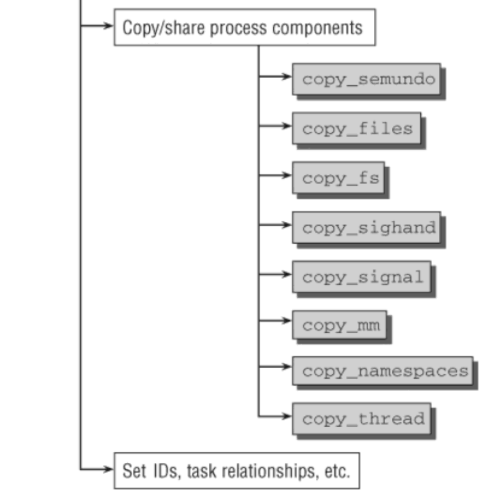
\includegraphics[width=.6\textwidth]{img/copy_process_2}
  \caption*{Схема работы copy\_process}
\end{figure}
\end{frame}	


\begin{frame}[fragile]
\frametitle{[Ядро 2.6.32][FORK] Анализ исходного кода}
Реализация также представлена в файле \textbf{fork.c}, по пути \textbf{/kernel/fork.c}.

Начало реализация представлено в строке 1166.
\lstinputlisting[firstnumber=1166,firstline=1166,lastline=1172, caption=.../kernel/fork.c]{sourceCode/kernel/2.6.32/kernel/fork.c}
\end{frame}	


\begin{frame}[fragile]
\frametitle{[Ядро 2.6.32][FORK] Анализ исходного кода}
Вся реализация уже описана для версии ядра 4.13, имеются следующие отличия:
\begin{enumerate}
\item у конструктора функции убран аргумент \textbf{tls} (определение локального хранилища);
\item убраны различные проверки флагов, которые ранее информировали \textbf{ptrace} о вызванном событии.
\end{enumerate}
В остальном, за исключением меньшего количество проверок входных данных, все идентично.
\end{frame}	


\begin{frame}[fragile]
\frametitle{[Ядро 2.6.32][FORK] Перехват вызова}
В файле по пути \textbf{/include/asm-generic/} имеется файл \textbf{syscalls.h}, в котором определен прототип fork().
\lstinputlisting[firstnumber=17,firstline=17,lastline=19, caption=.../kernel/asm-generic/syscalls.h]{sourceCode/kernel/2.6.32/asm-generic/syscalls.h}
\end{frame}	


\begin{frame}[fragile]
\frametitle{[Ядро 2.6.32][FORK] Перехват вызова}
Для того, чтобы перехватить данную функцию, напишем метод khook\_sys\_fork, который будет перехватывать системный вызов и перенаправлять управление нам:

\lstinputlisting[firstnumber=203,firstline=203,lastline=217, caption=Функция перехвата fork()]{sourceCode/fork/hookProgram/module-init.c}
\end{frame}	


\begin{frame}[fragile]
\frametitle{[Ядро 2.6.32][FORK] Сборка модуля}
Выполним Makefile для компиляции модуля ядра:
\lstinputlisting[caption=Лог сборки]{sourceCode/fork/hookProgram.logs/make.log}
\end{frame}	


\begin{frame}[fragile]
\frametitle{[Ядро 2.6.32][FORK] Операции с модулем}
Необходимые операции для работы:
\begin{enumerate}
\item \textbf{insmod} - вставка модуля в ядро (без полной перекомпиляции);
\item \textbf{lsmod} - просмтр списка текущий, работающих модулей;
\item \textbf{rmmod} - удаления заданного модуля.
\end{enumerate}
Операции должны быть произведены от пользователя с правами администратора.
\end{frame}	


\begin{frame}[fragile]
\frametitle{[Ядро 2.6.32][FORK] Проверка перехвата}
\lstinputlisting[caption=Лог с сообщением о перехвате, basicstyle=\fontsize{6}{6}\selectfont]{sourceCode/fork/hookProgram.logs/hook.log}
\end{frame}	


\begin{frame}[fragile]
\frametitle{[Ядро 2.6.32][FORK] Иерархия вызовов}
Дополнительно, если привести иерархию вызовов, то можно заметить что не только fork() и clone() используют функцию do\_fork().
\begin{figure}[H]
  \centering
  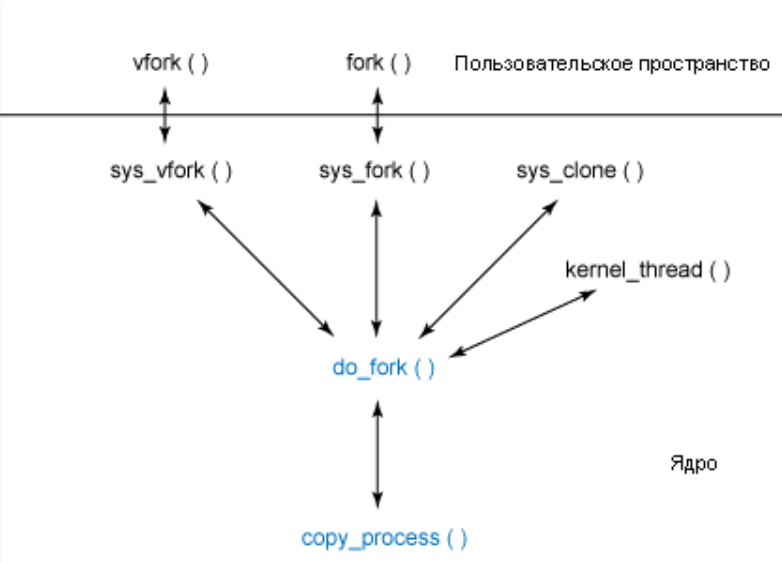
\includegraphics[width=.65\textwidth]{img/hierarchy}
  \caption*{Иерархия вызовов для do\_fork}
\end{figure}
\end{frame}	


\section{Системная функция execve}

\begin{frame}
\frametitle{Описание}
\textbf{execve()} - выполняет программу, задаваемую аргументом filename.\\
\textbf{Расположение: }.../fs/exec.c\\
\textbf{Синтаксис: } long sys\_execve(char \_\_user *filename, char \_\_user * \_\_user *argv, char \_\_user * \_\_user *envp, struct pt\_regs *regs)\\
Аргементы:
\begin{itemize}
\item \textbf{filename} - имя файла для выполнения;
\item \textbf{argv и envp} - вектор аргументов и среда выполнения;
\item \textbf{regs} - указатель на структуру регистров, на момент вызова данной функции.
\end{itemize}
\end{frame}


\begin{frame}[fragile]
\frametitle{Программы для анализа}
Программа печатает в консоль сообщение, часть которого передается в виде одно из аргументов запуска. Также, в цикле выводятся все переменные окружения. Для определения размера массива с переменными, согласно документации, последний элемент будет NULL.
\lstinputlisting[caption=sys\_execve.c, label={lst:execve}]{sourceCode/execve/programs/sys_execve.c}
\end{frame}	


\begin{frame}[fragile]
\frametitle{Вектор аргументов envp}
\lstinputlisting[firstnumber=28,firstline=28,lastline=46, numbers=none, caption=sys\_execve.log]{sourceCode/execve/kernels/4.13/sys_execve.log}
\end{frame}	


\begin{frame}[fragile]
\frametitle{[Ядро 4.13.0][EXECVE] STRACE}
Для сокращения лога, приведены первые 2 строчки лога strace.
\lstinputlisting[firstnumber=1,firstline=1,lastline=2, caption=sys\_execve\_strace.log]{sourceCode/execve/kernels/4.13/sys_execve_strace.log}
Аргументы соответствуют ожиданиям, первый аргумент соответствует программе для запуска. Далее расположен массив аргументов, передаваемых в запускаемую программу. И наконец передаются переменные окружения, правда в данном случае, из-за их обилия они скрыты, и показано лишь их количество.
\end{frame}	


\begin{frame}[fragile]
\frametitle{[Ядро 4.13.0][EXECVE] Анализ исходного кода}
Основная часть, архитектурно независимого кода находится в файле \textbf{exec.c} по пути \textbf{/fs/}.
\lstinputlisting[firstnumber=1828,firstline=1828,lastline=1835, caption=../fs/exec.c]{sourceCode/kernel/4.13/fs/exec.c}
\end{frame}	


\begin{frame}[fragile]
\frametitle{[Ядро 4.13.0][EXECVE] Анализ исходного кода}
Если сравнивать с ядром керсии 2.6.32, то в данном случае, оригинальная функция \textbf{do\_execve} превратилась в некоторую обертку, а основная функциональность была перенесена в функцию \textbf{do\_execveat\_common}.
\lstinputlisting[firstnumber=1679,firstline=1679,lastline=1686, caption=../fs/exec.c]{sourceCode/kernel/4.13/fs/exec.c}
\end{frame}	


\begin{frame}[fragile]
\frametitle{[Ядро 4.13.0][EXECVE] Принцип работы}
\begin{figure}[H]
  \centering
  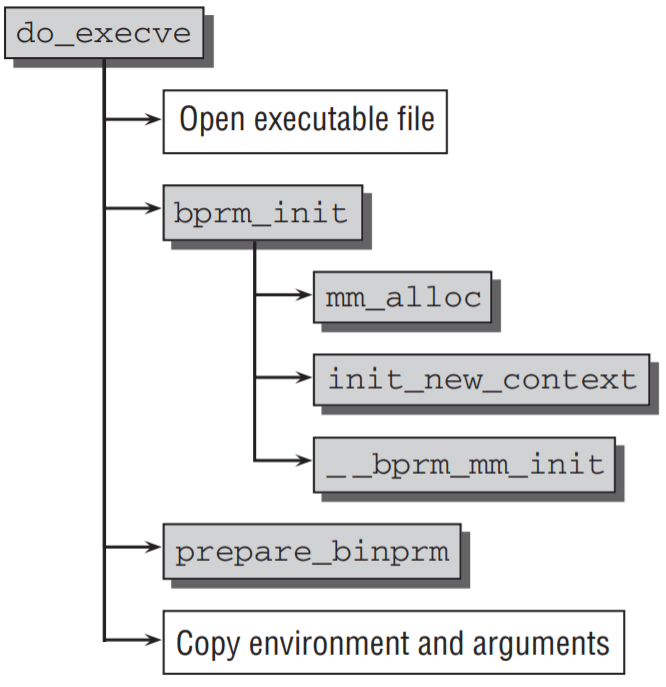
\includegraphics[width=.6\textwidth]{img/do_execve}
  \caption*{Схема работы do\_execve}
\end{figure}
\end{frame}	


\begin{frame}[fragile]
\frametitle{[Ядро 2.6.32][EXECVE] Анализ исходного кода}
Основная часть, архитектурно независимого кода находится в файле \textbf{exec.c} по пути \textbf{/fs/}.
\lstinputlisting[firstnumber=1069,firstline=1069,lastline=1076, caption=../fs/exec.c]{sourceCode/kernel/2.6.32/fs/exec.c}
В отличии от ядра 4.13, в данном случае никакой обертки над функцией нет. По коду, основным отличием является то, что отдельные функции из \textbf{bprm\_init} были перенесены непосредственно в тело функции \textbf{do\_execve}.
\end{frame}	


\begin{frame}[fragile]
\frametitle{[Ядро 2.6.32][EXECVE] Перехват вызова}
В файле по пути \textbf{/include/asm-generic/} имеется файл \textbf{syscalls.h}, в котором определен прототип execve().
\lstinputlisting[firstnumber=25,firstline=25,lastline=28, caption=.../kernel/asm-generic/syscalls.h]{sourceCode/kernel/2.6.32/asm-generic/syscalls.h}
\end{frame}	


\begin{frame}[fragile]
\frametitle{[Ядро 2.6.32][EXECVE] Перехват вызова}
Для того, чтобы перехватить данную функцию, напишем метод khook\_sys\_execve, который будет перехватывать системный вызов и перенаправлять управление нам:
\lstinputlisting[firstnumber=203,firstline=203,lastline=218, caption=Функция перехвата execve()]{sourceCode/execve/hookProgram/module-init.c}
\end{frame}	


\begin{frame}[fragile]
\frametitle{[Ядро 2.6.32][EXECVE] Проверка перехвата}
\lstinputlisting[caption=Системный лог, basicstyle=\fontsize{6}{6}\selectfont]{sourceCode/execve/hookProgram.logs/kern.log}
\end{frame}	


\section{Системная функция exit}
\begin{frame}
\frametitle{Описание}
\textbf{exit()} - завершает работу программы. Все дескрипторы файлов, принадлежащие процессу, закрываются; все его дочерние процессы начинают управляться процессом 1 (init), а родительскому процессу посылается сигнал SIGCHLD.\\
\textbf{Расположение: }.../kernel/exit.c\\
\textbf{Синтаксис: } long sys\_exit(int error\_code)\\
Аргементы:
\begin{itemize}
\item \textbf{error\_code} - код выхода.
\end{itemize}
\end{frame}


\begin{frame}[fragile]
\frametitle{Программы для анализа}
Программа выводит в консоль два сообщения, одно до, а другое после системного вызова exit, по коду 60 (системный номер функции).
\lstinputlisting[caption=sys\_exit.c, label={lst:exit}]{sourceCode/exit/programs/sys_exit.c}
\end{frame}	


\begin{frame}[fragile]
\frametitle{[Ядро 4.13.0][EXIT] STRACE}
\lstinputlisting[firstnumber=25,firstline=25,lastline=33, caption=sys\_exit\_strace.log]{sourceCode/exit/kernels/4.13/sys_exit_strace.log}
Внимания стоит уделить строчкам 30 и 32. В строчке 30 происходит вывод текста в консоль, а далее, в строке 32 происходит вызов систеного вызова exit, после которого, никаких других сисмных вызовов не последовало.
\end{frame}	


\begin{frame}[fragile]
\frametitle{[Ядро 4.13.0][EXIT] Анализ исходного кода}
Основная часть, архитектурно независимого кода находится в файле \textbf{exit.c} по пути \textbf{/kernel/}. Далее приведено лишь начало функции \textbf{do\_exit}.
\lstinputlisting[firstnumber=763,firstline=763,lastline=777, caption=../kernel/exit.c]{sourceCode/kernel/4.13/kernel/exit.c}
\end{frame}	


\begin{frame}[fragile]
\frametitle{[Ядро 4.13.0][EXIT] Принцип работы}
\begin{enumerate}
\item В вызвавшем процессе закрываются все дескрипторы открытых файлов;
\item Если родительский процесс находится в состоянии вызова wait, то системный вызов wait завершается, выдавая родительскому процессу в качестве результата идентификатор терминировавшегося процесса;
\item Если родительский процесс не находится в состоянии вызова wait, то процесс, вызвавший exit, переходит в состояние зомби.  Элемент таблицы процессов, занятый зомби-процессом, содержит информацию о времени, затраченном процессом.
\end{enumerate}
У всех существующих потомков терминировавшихся процессов, а также у зомби-процессов идентификатор родительского процесса устанавливается равным 1. Таким образом, все эти процессы наследуются инициализационным процессом.
\end{frame}	


\begin{frame}[fragile]
\frametitle{[Ядро 4.13.0][EXIT] Некоторые вызываемые функции}
\begin{itemize}
\item \textbf{exit\_sem()} - если процесс находится в очереди в ожидании семафора IPC, то он выгружается.
\item \textbf{\_\_exit\_files(), \_\_exit\_fs(), exit\_namespace(), и exit\_sighand()} - уменьшения показателя использования объектов связанных с файловыми дескрипторами, данными файловой системы, пространством имен процессов и обработчиками сигналов. Если какой-либо показатель использования достигает нуля, объект больше не используется каким-либо процессом и удаляется.
\item \textbf{exit\_notify()} - отправка сигнала о завершении процесса родительскому и всем(если имеются) дочерним процессам. Перевод процесса в состояние зомби.
\end{itemize}
\end{frame}	


\begin{frame}[fragile]
\frametitle{[Ядро 2.6.32][EXIT] Анализ исходного кода}
Как и у ядра 4.13, основная часть кода расположена в файле \textbf{exit.c}, а далее приведено начало функции \textbf{do\_exit}.
\lstinputlisting[firstnumber=796,firstline=796,lastline=802, caption=../kernel/exit.c]{sourceCode/kernel/2.6.32/kernel/exit.c}
Вся реализация, подобна реализации в ядре 4.13, за исключением того, что в данном случае, порядок действий в несколько ином порядке, а также уменьшено количество действий по обеспечению откладочной информации, например отсутствует нотификация ptrace.
\end{frame}	


\begin{frame}[fragile]
\frametitle{[Ядро 2.6.32][EXIT] Перехват вызова}
В файле по пути \textbf{/include/linux/} имеется файл \textbf{syscalls.h}, в котором определен прототип exit().
\lstinputlisting[firstnumber=418,firstline=418,lastline=418, caption=.../kernel/linux/syscalls.h]{sourceCode/kernel/2.6.32/linux/syscalls.h}
\end{frame}	


\begin{frame}[fragile]
\frametitle{[Ядро 2.6.32][EXIT] Перехват вызова}
Для того, чтобы перехватить данную функцию, напишем метод khook\_sys\_exit, который будет перехватывать системный вызов и перенаправлять управление нам:
\lstinputlisting[firstnumber=203,firstline=203,lastline=218, caption=Функция перехвата exit()]{sourceCode/exit/hookProgram/module-init.c}
\end{frame}	


\begin{frame}[fragile]
\frametitle{[Ядро 2.6.32][EXIT] Проверка перехвата}
\lstinputlisting[caption=Системный лог]{sourceCode/exit/hookProgram.logs/kern.log}
\end{frame}	


\section{Модификация системных вызовов}

\begin{frame}[fragile]
\frametitle{[Ядро 4.13.0][FORK] Вносимая модификация}
В начале основной функции \textbf{do\_fork}(файл \textbf{/kernel/fork.c}) было добавлено информационное сообщение(строка 2016) для записи в системный лог.
\lstinputlisting[firstnumber=2006,firstline=2006,lastline=2017, caption=Модифицированный fork]{sourceCode/modification/modifiedUtils/fork.c}
\end{frame}	


\begin{frame}[fragile]
\frametitle{[Ядро 4.13.0][EXECVE] Вносимая модификация}
\lstinputlisting[firstnumber=1682,firstline=1682,lastline=1696, caption=Модифицированный exec]{sourceCode/modification/modifiedUtils/exec.c}
Сразу после успешной проверки на валидность файла(строка 1693), происходит вывод информационного сообщения(строка 1696).
\end{frame}	


\begin{frame}[fragile]
\frametitle{[Ядро 4.13.0][EXIT] Вносимая модификация}
В начале основной функции \textbf{do\_exit}(файл \textbf{/kernel/exit.c}) было добавлено информационное сообщение(строка 765) для записи в системный лог.
\lstinputlisting[firstnumber=763,firstline=763,lastline=765, caption=Модифицированный exit]{sourceCode/modification/modifiedUtils/exit.c}
\end{frame}	

\section{Перекомпиляция ядра}

\begin{frame}[fragile]
\frametitle{Подготовка к компиляции}
\begin{enumerate}
\item Скачать интересующее ядро по ссылке, в данном случае 4.13.0
\begin{lstlisting}[numbers=none]
https://mirrors.edge.kernel.org/pub/linux/kernel/v4.x/
\end{lstlisting}
\item Далее необходимо установить некоторые пакеты следующей командой:
\lstinputlisting[numbers=none]{sourceCode/modification/guide/install_1.log}
\item Распаковать архив с исходным кодом по пути \textbf{/usr/src/}.
\end{enumerate}
\end{frame}	


\begin{frame}[fragile]
\frametitle{Конфигурация ядра}
Выполним команду: \textbf{sudo make menuconfig}
\begin{figure}[H]
  \centering
  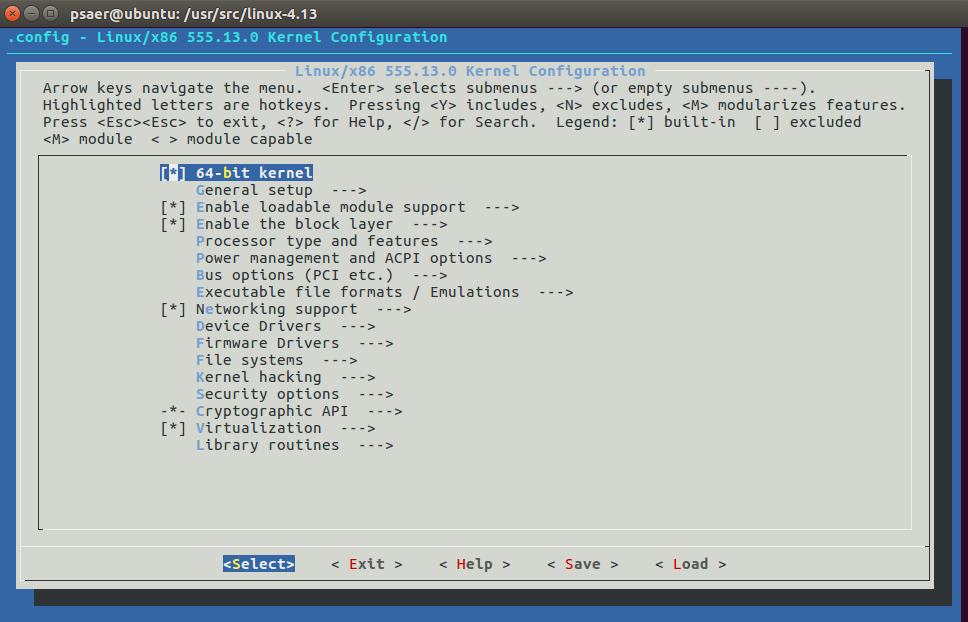
\includegraphics[width=.85\textwidth]{img/menuconfig}
  \caption*{Конфигурация ядра}
\end{figure}
\end{frame}	


\begin{frame}[fragile]
\frametitle{Настройка makefile}
Перед компиляцией ядра, внесем изменения в файл \textbf{Makefile}, который находится в корне разархивированного ядра.
\lstinputlisting[firstnumber=1,firstline=1,lastline=5,caption=Файл Makefile]{sourceCode/modification/Makefile.txt}
В представленных первых 5 строках представлена основная информация о версии ядра. В моем случае, вместо версии 4 была поставлена версия 555.
\end{frame}	


\begin{frame}[fragile]
\frametitle{Компиляция ядра}
Теперь приступаем к компиляции, для этого выполняем следующую команду:
\lstinputlisting[caption=Компиляция ядра]{sourceCode/modification/guide/install_3.log}
Ключ \textbf{j} означает количество задействованных ядер системы. В моем случае, в настройках VMware, виртуальной машине было выделено 3 ядра процессора.

Первые две команды, из листинга выше, выполняют компиляцию ядра, а последняя компилирует въедино в образ ядра системы.

Процесс, в моем случае занимиает около 20 минут.
\end{frame}	


\begin{frame}[fragile]
\frametitle{Настройка GRUB}
Далее необходимо включить показ меню \textbf{GRUB}. Для этого редактируем файл \textbf{grub} по пути \textbf{/etc/default/}.
\lstinputlisting[firstnumber=1,firstline=1,lastline=10, caption=Файл grub]{sourceCode/modification/grub.txt}
В данном файле необходимо закомментировать(поставить знак \# в начале строки) строки 7 и 8.
\end{frame}	


\begin{frame}[fragile]
\frametitle{Меню GRUB}
\begin{figure}[H]
  \centering
  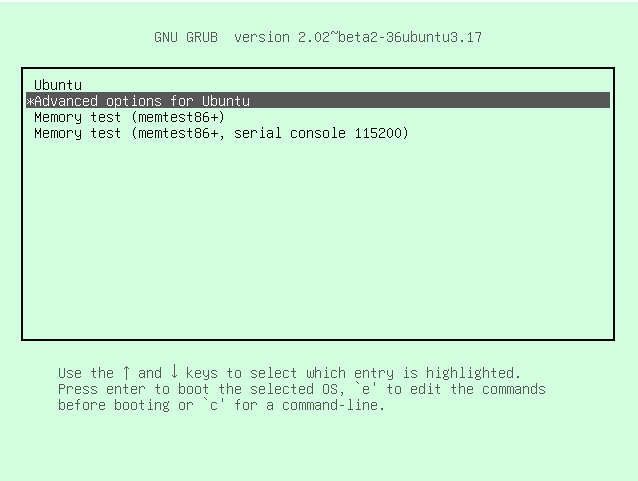
\includegraphics[width=.85\textwidth]{img/grub_1}
  \caption*{Меню GRUB}
\end{figure}
\end{frame}	


\begin{frame}[fragile]
\frametitle{Выбор ядра в GRUB}
\begin{figure}[H]
  \centering
  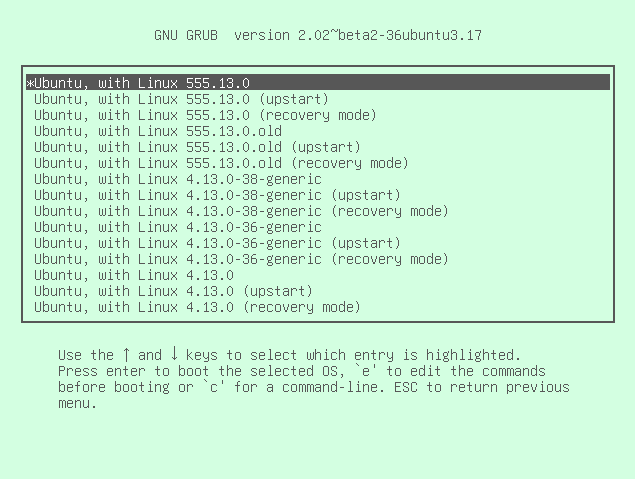
\includegraphics[width=.8\textwidth]{img/grub_2}
  \caption*{Выбор ядра в GRUB}
\end{figure}
\end{frame}	


\begin{frame}[fragile]
\frametitle{Проверка модификации}
Выполним программу, напрямую вызывающую fork.
\lstinputlisting[caption=Выполнением программы с прямым вызовом fork]{sourceCode/modification/check/fork.log}

Для поиска сообщений, которые записываются в системный лог, будет использована следующая команда:
\lstinputlisting[firstnumber=1,firstline=1,lastline=1,caption=Команда для поиска некоторого сообщения]{sourceCode/modification/check/fork.txt}
Поиск происходит рекурсивно, в каталоге \textbf{/var/log/} на предмет наличия в тексте \textbf{fork}.
\end{frame}	


\begin{frame}[fragile]
\frametitle{Проверка модификации}
\lstinputlisting[firstnumber=122,firstline=122,lastline=130,caption=Результаты поиска fork]{sourceCode/modification/check/fork.txt}
\end{frame}	


\begin{frame}[fragile]
\frametitle{Проверка модификации}
\lstinputlisting[caption=Результаты поиска exit, basicstyle=\fontsize{6}{6}\selectfont]{sourceCode/modification/check/exit.txt}
\end{frame}	




\begin{frame}
\frametitle{Список источников}
\begin{itemize}
\item Writing a Linux Kernel Module. –– URL: http://derekmolloy.ie/writing-a-linux-kernel-module-part-1-introduction/ (дата обращения: 2018-04-06).\\
\item Встраивание в ядро Linux: перехват функций. –– URL: https://habrahabr.ru/ company/securitycode/blog/237089/ (дата обращения: 2018-04-07).\\
\item fork(2) - Linux man page. –– URL: https://linux.die.net/man/2/fork (дата обращения: 2018-04-01).\\
\item clone(2) - Linux man page. –– URL: https://linux.die.net/man/2/clone (дата обращения: 2018-04-01).\\
\item glibc, archive of versions. –– URL: https://ftp.gnu.org/gnu/glibc/ (дата обращения: 2018-04-04).\\
\end{itemize}


\end{frame}


\begin{frame}
\frametitle{Список источников}
\begin{itemize}
\item Fork bomb. –– URL: https://en.wikipedia.org/wiki/Fork\_bomb (дата обращения: 2018-04-07).\\
\item execve - execute program. –– URL: http://man7.org/linux/man-pages/man2 execve.2.html (дата обращения: 2018-04-08).\\
\item exit – terminate process. –– URL: http://man.cat-v.org/unix-1st/2/sys-exit (дата обращения: 2018-04-08).\\
\item Анатомия управления процессами в Linux. –– URL: https://www.ibm.com/ developerworks/ru/library/l-linux-process-management/index.html (дата обращения: 2018-04-07).
\end{itemize}
\end{frame}


\end{document}
